\subsection{Arquitectura de EfficientNet-B3}

EfficientNet-B3 es una red neuronal convolucional cuyo funcionamiento sigue el flujo clásico de una CNN: las imágenes de entrada pasan por sucesivas capas que extraen patrones visuales de forma progresiva, desde características simples como bordes y texturas hasta representaciones más complejas, para finalmente producir una clasificación.

Lo que distingue a EfficientNet-B3 de una CNN convencional son tres elementos clave en su diseño. Primero, su bloque fundamental es el \textbf{MBConv} (\textit{Mobile Inverted Bottleneck Convolution}), que reemplaza la convolución clásica separando la detección de patrones espaciales de la combinación de canales, logrando la misma capacidad representativa con un menor costo computacional. Segundo, cada bloque MBConv incorpora un mecanismo de \textbf{Squeeze-and-Excitation}, que pondera la importancia de cada canal de forma adaptativa según el contenido de la imagen, amplificando las características más relevantes y suprimiendo las irrelevantes. Tercero, la arquitectura base fue obtenida mediante \textbf{búsqueda de arquitectura neuronal} (NAS), lo que garantiza que el punto de partida ya sea óptimo antes de aplicar cualquier escalado.

A partir de esta base (EfficientNet-B0), el modelo B3 se obtiene aplicando \textbf{Compound Scaling}: un método que escala simultáneamente la profundidad (número de capas), el ancho (número de filtros por capa) y la resolución de entrada, en proporción balanceada. Esto contrasta con enfoques tradicionales que escalan solo una dimensión, y explica por qué EfficientNet-B3 alcanza un 81.6\% de precisión en ImageNet con apenas 12.3~M de parámetros.

\begin{figure}[H]
    \centering
    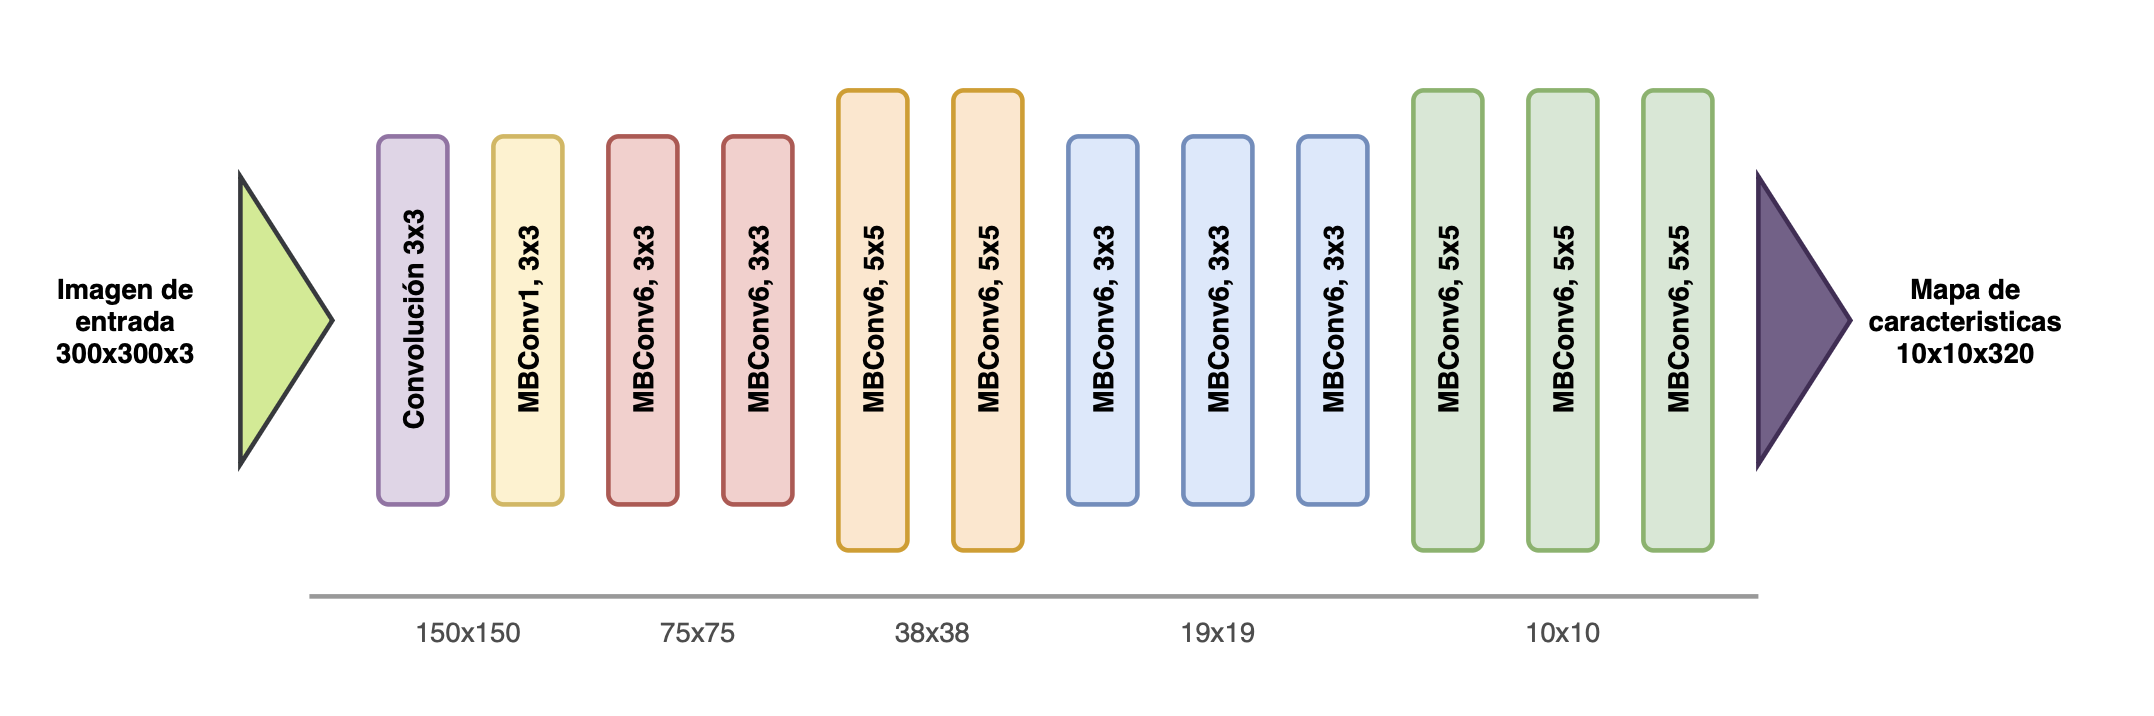
\includegraphics[width=1\textwidth]{images/C5/arq.png}
    \caption{Arquitectura CNN de EfficientNet.}
    \label{fig:arquitecturaEfficientNet}
\end{figure}
